\chapter{HTML5 egitura-osagaiak}

Hainbat etiketa semantiko berri aurki ditzakegu HTML5en  \href{https://html.spec.whatwg.org/multipage/sections.html}{espezifikazioan}\footnote{https://html.spec.whatwg.org/multipage/sections.html}. Horietatik, garrantzitsuenak eta askotan erabiltzen direnak, \textit{header}, \textit{footer}, \textit{nav}, \mbox{\textit{article}}, \textit{section} eta \textit{aside} dira.

\index{header}
Deskribapen eta eztabaida sakon eta aspergarri bat eman ordez, hobe iruditu zait adibideekin aztertzea. Dena den, etiketa garrantzitsu horien deskribapen oso labur batekin hasiko gara.
% <header>  <footer> <nav> <article> <section> <aside> 


\textbf{<header>} Webgunearen goiburua irudikatzeko etiketa. 

\index{footer}
\textbf{<footer>} Webgunearen orri-oina irudikatzeko etiketa. Adi, ez da beti orriaren beheko aldean zertan agertu. 

\index{nav}
\textbf{<nav>} Webgunetik nabigatzeko menua (edo antzeko funtzionalitatea) gordeko du.

\index{article}
\textbf{<article>} Bere baitan zentzua daukan eduki puska gordeko du. Etiketa honen barruan gordetzen dugun edukiak zentzua izan beharko luke RSS jario baten elementu gisa (adibidez, egunkari baten berriak emateko RSS baten barruan, berri-laburpen bat <article> bat izan daiteke)

\index{section}
\textbf{<section>} Artikuluak (<article> osagaiak) gaiaren arabera multzokatzeko erabil daitezke, baina baita artikulu baten barruan dagozkion atalak zehazteko ere.

\index{aside}
\textbf{<aside>} Alboko edukiak eduki bloke bat zehazten du, bere inguruan dagoen eduki nagusiarekin zerikusia duen zerbait gordetzeko (baina eduki nagusiaren jarioarekin guztiz bat ez datorren zerbait).

\begin{figure}[ht]
	\centering
\begin{tikzpicture}
\node[anchor=south west,inner sep=0] (image) at (0,0)
   {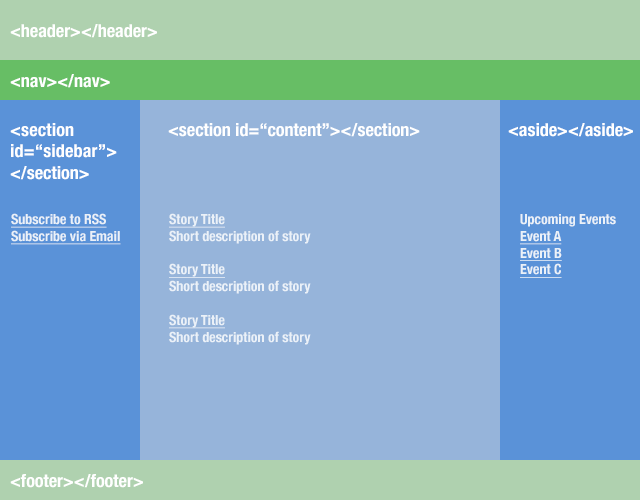
\includegraphics[trim=0cm 0cm 0cm 0cm, clip=true, width=0.75\textwidth]{img/structural_content}};
%    \begin{scope}[x={(image.south east)},y={(image.north west)}]
% \fill[color=red] (0.503, 0.44) rectangle(0.533, 0.685);
%\end{scope}
\end{tikzpicture}
\caption{HTML5 egitura-osagaiak. Iturria: \href{http://stackoverflow.com/a/24765186/243532}{http://stackoverflow.com/a/ 24765186/243532}.}
\label{fig:html5etiketasematikoak}
\end{figure}

Goazen adibideetara. Lehenengoa, nola ez, \href{http://stackoverflow.com/a/24765186/243532}{StackOverflow webgunetik}\footnote{http://stackoverflow.com/a/24765186/243532} hartua da eta \ref{fig:html5etiketasematikoak}. irudian ikus dezakegu. Bertan orri baten goiburua adierazteko \textit{header} etiketa erabiltzen dela adierazten dugu. Ildo beretik, askotan nabigatzeko barra bat ikusten da, \textit{nav} etiketekin adierazita irudian. Orri baten atal nagusiak, edukia bera eta dokumentuaren azpiataletik nabigatzeko esteka zuzenak, \textit{section} etiketen barruan sartuko ditugu. Uneko dokumentuarekin lotura zuzena ez baina zeharkako lotura duen beste eduki bat kodean antolatzeko, \textit{aside} etiketa erabil dezakegu. Bukatzeko, orri-oinak \textit{footer} gisa markatuko ditugu. Aipatutakoa, antolaketa modu bat da, W3Ck gomendatzen duena hain zuzen ere, baina kontuz, zenbait xehetasun daude. Alde batetik, \textit{footer} etiketaren edukiak ez du beti dokumentuaren beheko aldean agertu behar, baliteke beste oin batzuk izatea. \textit{Section} baten barruan artikulu (\textit{article}) batzuk izan ditzakegu... eta alderantziz! Ikus ditzagun adibide zehatz batzuk hau guztia ondo barneratzeko.

\begin{figure}[ht]
	\centering
\begin{tikzpicture}
\node[anchor=south west,inner sep=0] (image) at (0,0)
   {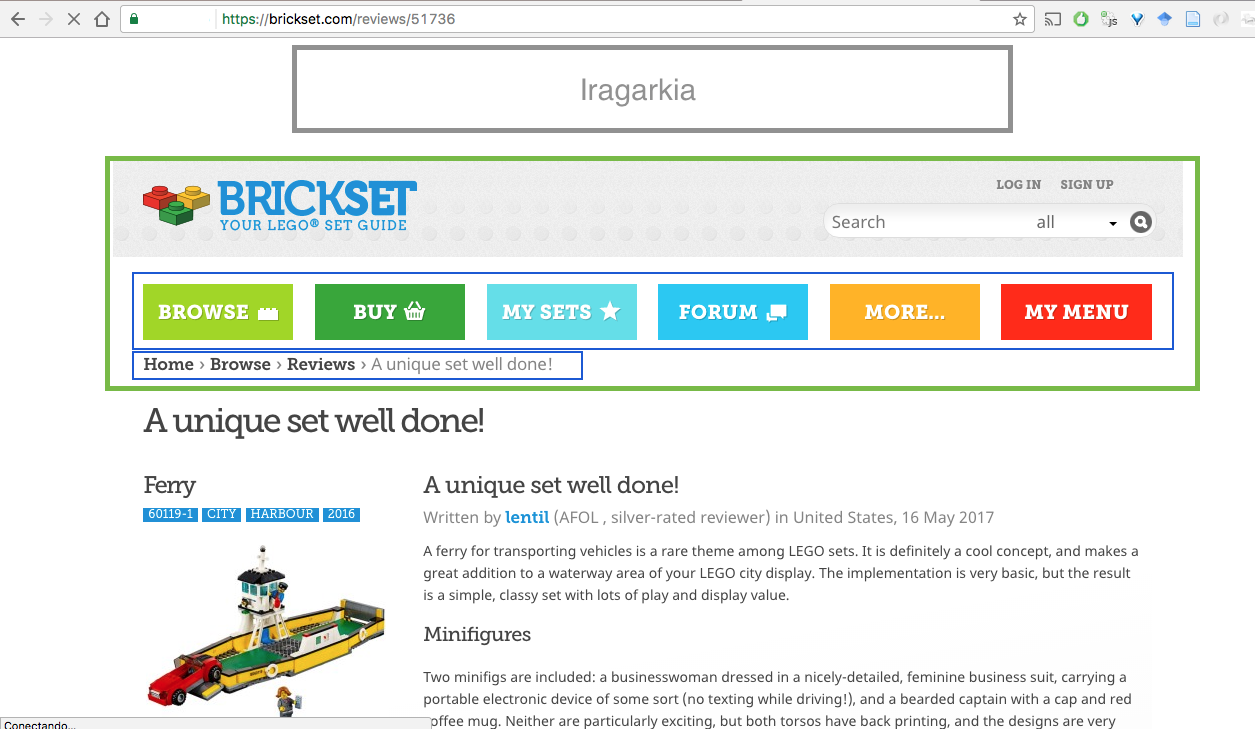
\includegraphics[trim=0cm 0cm 0cm 0cm, clip=true, width=.75\textwidth]{img/lego_html}};
\end{tikzpicture}
\caption{HTML5 egitura-osagaiak.}
\label{fig:legohtml5etiketak}
\end{figure}

\begin{figure}[ht]
	\centering
\begin{tikzpicture}
\node[anchor=south west,inner sep=0] (image) at (0,0)
   {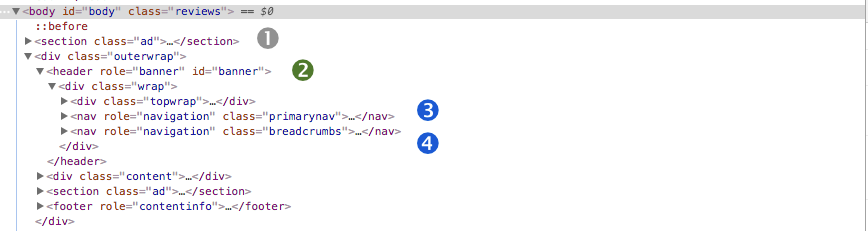
\includegraphics[trim=0cm 0cm 0cm 0cm, clip=true, width=\textwidth]{img/html_kodea}};
\end{tikzpicture}
\caption{HTML5 etiketa semantikoak: Lego orriaren adibidea. Kodea.}
\label{fig:legohtml5etiketakkodea}
\end{figure}


Adibidez, har dezagun  \href{https://brickset.com/reviews/51736}{Lego webgunearen orri bat}\footnote{https://brickset.com/reviews/51736},  \ref{fig:legohtml5etiketak}. irudian ikus dezakeguna. Orriari dagokion HTML kodea  \ref{fig:legohtmledukiakodea} irudian daukagu. Bertan 1. puntuan (grisez), \textit{section} bat aurkitzen dugu, orriaren iragarkia edo \textit{banner-a} adierazteko. Jarraian, 2. puntuan, \textit{header} etiketa, Lego webgunetik nabigatu ahal izateko botoiak, bilatzailea eta ogi-papurren bidea adierazteko. Goiburuaren (\textit{header-}en) barruan, bi \textit{nav} etiketa, nabigatzeko lehenengo botoi-barra eta ogi-papurren bidea markatzeko.

\begin{figure}[ht]
	\centering
\begin{tikzpicture}
\node[anchor=south west,inner sep=0] (image) at (0,0)
   {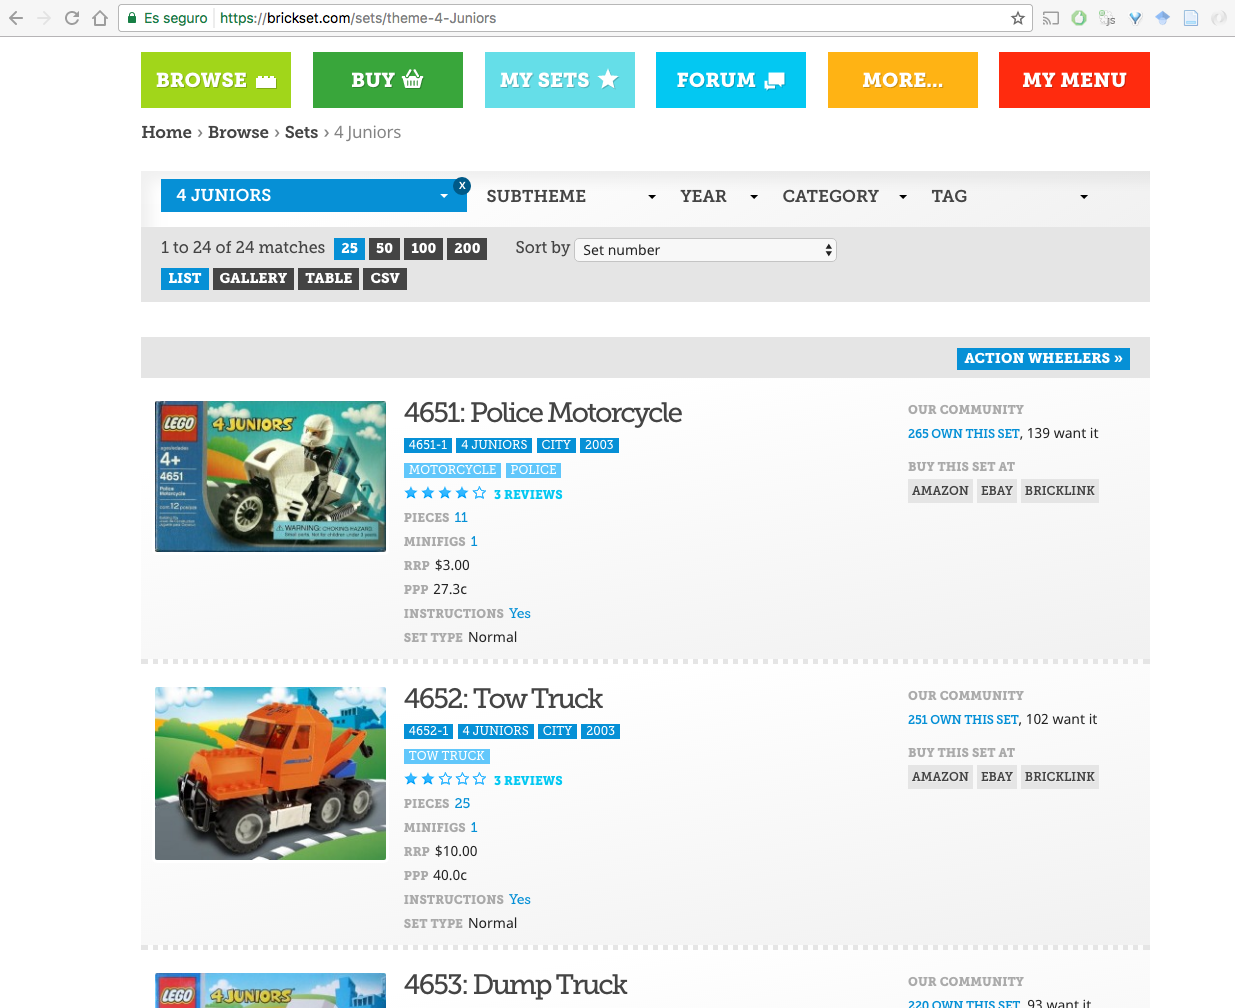
\includegraphics[trim=0cm 0cm 0cm 0cm, clip=true, width=.75\textwidth]{img/lego_content}};
\end{tikzpicture}
\caption{HTML5 egitura-osagaiak. Eduki nagusia.}
\label{fig:legohtml5edukia}
\end{figure}

\begin{figure}[ht]
	\centering
\begin{tikzpicture}
\node[anchor=south west,inner sep=0] (image) at (0,0)
   {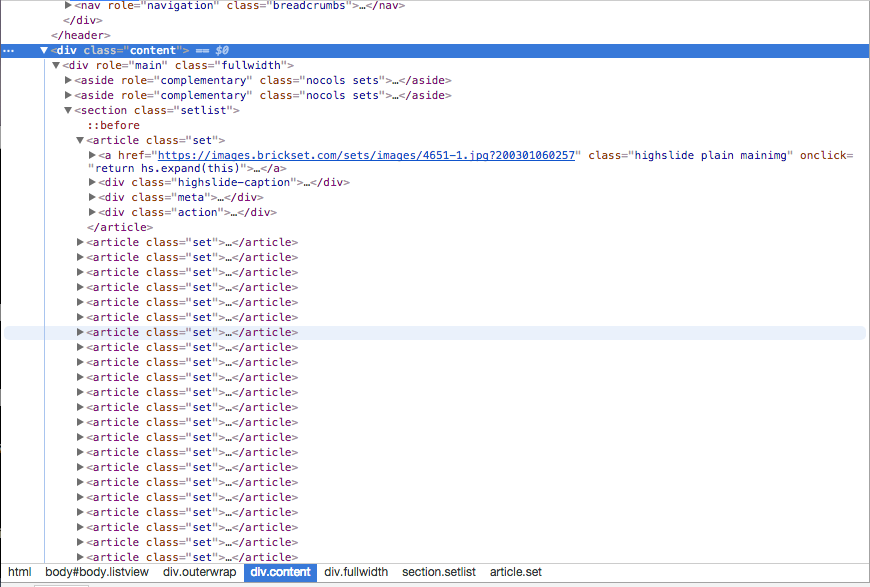
\includegraphics[trim=0cm 0cm 0cm 0cm, clip=true, width=0.75\textwidth]{img/lego_content_kodea}};
\end{tikzpicture}
\caption{HTML5 etiketa semantikoak: Lego orriaren adibidea (II). Kodea.}
\label{fig:legohtmledukiakodea}
\end{figure}

Lego bilduma-bilatzailean sartuz gero, goiburua (\textit{header}) berdina bada ere, edukia noski, aldatzen da (ikus \ref{fig:legohtml5edukia}. irudia). Eduki horri dagokion kodea \ref{fig:legohtmledukiakodea}. irudian aztertuko dugu. Bertan, bi \textit{aside} daude, figura-bildumetatik nabigatzeko eta iragazketa egiteko inprimakiekin. Jarraian, \textit{section} etiketaren barruan, figura-bilduma guztiak, banan-banan, bakoitza \textit{article} etiketa baten barruan.

\section{Ariketak}

\begin{enumerate}

\item Ordezkatu <div> etiketa bakoitza dagokion HTML5 etiketa semantiko egokiaz:
 
 \begin{lstlisting}[language=HTML,numbers=none]
 <div id="header">
<h1> Goi mailako goiburu bat naiz</h1
</div>
<div id="footer">
 <h3> UPV/EHU </h3>
 <p> 2020/21 ikasturtea </p>
</div>
 \end{lstlisting}
 
 
\item Ordezkatu <div> etiketa bakoitza dagokion HTML5 etiketa semantiko egokiaz:

 \begin{lstlisting}[language=HTML,numbers=none]
 <div id="navigation">
<ul>
<li>Euskal Herrian</li>
<li>Datuak munduan</li>
<li>Shock ekonomikoa</li>
<li>Buletin berezia</li>
</ul>
</div>
  \end{lstlisting}
 
 \item Ordezkatu <div> etiketa bakoitza dagokion HTML5 etiketa semantiko egokiaz eta bihurtu goiburu-etiketak h1 eta h2:

\begin{lstlisting}[language=HTML,numbers=none]
<div class="section">
 <h2>Berrinfekzio kasuen berri eman dute Belgikan eta
Herbehereetan ere</h2>
 <h3>OME Osasunaren Mundu Erakundearen iritzia</h3>
 <p>Astelehenean jakin zen COVID-19 birusarekin berrinfektutako
pertsona bat atzeman zutela lehen aldiz...</p>
</div>
 \end{lstlisting}
 
 \item Gehitu beharrezko <article> etiketak:
 \begin{lstlisting}[language=HTML,numbers=none]
 <section id="koronabirusa">
<header>
 <h1>Eguneraketa</h1>
</header>
 <h2>Osasun sistemaren gaitasuna</h2>
 <p>Urkulluren ustez, osasun sistemaren gaitasuna ''bermaturik''
dago</p>
 <h2>Berrinfekzioak</h2>
 <p>Berrinfekzio kasuen berri eman dute Belgikan eta Herbehereetan
ere</p>
</section>
\end{lstlisting}

\item Ordezkatu <p class=\textquotedbl{}aside\textquotedbl{}> etiketa dagokion HTML5eko osagai egokiaz:

\begin{lstlisting}[language=HTML,numbers=none]
<section id="koronabirusa">
<header>
 <h1>Eguneraketa</h1>
</header>
<article>
 <h2>Osasun sistemaren gaitasuna</h2>
 <p>Urkulluren ustez, osasun sistemaren gaitasuna 
 ''bermaturik''
dago</p>
 <p class="aside">Pedro Sanchez Espainiako Gobernuko presidenteak ere agerraldia egin zuen atzo...</p>
</article>
</section>

\end{lstlisting}

\item 

Bihurtu HTML5 formatura HTML4n programatutako
adibide hau:

\begin{lstlisting}[language=HTML,numbers=none]

<!DOCTYPE html PUBLIC "-//W3C//DTD XHTML 1.0 Strict//EN"
"http://www.w3.org/TR/xhtml1/DTD/xhtml1-strict.dtd">
<html xmlns="http://www.w3.org/1999/xhtml"
 lang="eu_ES"
 xml:lang="eu_ES">
 <head>
 <meta charset="utf-8" />
 <title>1. Ariketa</title>
 <link href="css/style.css" rel="stylesheet" />
 </head>
 <body>
<div id="header">
<h1> Koronabirusa</h1
<h2>Euskal Herrian eta Munduan</h2>
</div>
<div id="navigation">
 <ul>
 <li>Euskal Herrian</li>
 <li>Datuak munduan</li>
 <li>Shock ekonomikoa</li>
 <li>Buletin berezia</li>
 </ul>
</div>
<div id="section">
 <h2>Zelaa aztertzen ari da COVID-19a duten haurren gurasoei
gaixo agiria ematea</h2>
<div class="article">
 <h3>Bihar elkartuko dira autonomia erkidegoetako
ordezkariekin</h3>
 <p>Maskarak, gel hidroalkoholikoak, PCRak, distantzia...
Funtsean, COVID-19ak baldintzatuko du 2020-2021eko ikasturtea.</
p>
 <p class="aside">Bihar bilera: Zelaak azaldu duenez, bihar
elkartuko dira autonomia erkidegoetako ordezkariekin</p>
</div>
<div class="article">
 <h3>Berrinfekzio kasuen berri eman dute Belgikan eta
Herbehereetan ere</h3>
 <p>
 OME Osasunaren Mundu Erakundeak esan du berrinfekzioen
gaineko berriak oraindik ''anekdotikoak'' direla, eta zer ikertua
franko dagoela
 </p>
</div>
</div>
<div id="footer">
 <h3> UPV/EHU </h3>
 <p> 2020/21 ikasturtea </p>
</div>
</body>
</html>
\end{lstlisting}

\item Bihurtu HTML5 formatura HTML4n programatutako
adibide hau:

\begin{lstlisting}[language=HTML,numbers=none]

<!DOCTYPE html PUBLIC "-//W3C//DTD HTML 4.01//EN"
"http://www.w3.org/TR/html4/strict.dtd">
<html>
<head>
<meta http-equiv="content-type" content="text/html; charset=UTF-8">
<title>Taberna</title>
<link type="text/css" rel="stylesheet" href="taberna.css">
<script type="text/javascript" src="taberna.js"></script>
</head>
<body>
<h1>Ongi Etorri Tabernara</h1>
<p>
<img src="edariak.gif" alt="Edariak">
</p>
<p>
Arratsaldero elkartzen gara xake edo mus partida batzuk jolastera <a
href="garagoardoak.html">garagardo batzuk</a> edaten dugun bitartean,
solasaldi ederraz gozatuz. WiFi sarea ere badugu, konexio on batekin.
</p>
</body>
</html>
\end{lstlisting}
\end{enumerate}
